% generated by paper/make_figures.py from results/rev2 - do not edit
\appendix
\section{Supplementary Measurement Figures}
\label{app:figs}
Figs.~\ref{fig:app-tcp}--\ref{fig:app-newconn} plot the measurements behind Tables~\ref{tab:perf} and \ref{tab:paths} with their 95\% confidence intervals (Student $t$). Value axes are zoomed so that the intervals are visible; each caption gives the axis origin, and differences between bars should be judged against the intervals, not against the axis origin. Table~\ref{tab:figindex} lists every figure with its quantity, the configurations it covers and its data file in the results directory (\texttt{results/rev2}).

\begin{table}[!h]
\caption{Index of the supplementary figures}
\label{tab:figindex}
\centering\scriptsize
\setlength{\tabcolsep}{3pt}
\begin{tabular}{@{}rlll@{}}
\toprule
Fig. & Name & Unit & Configurations \\
\midrule
\ref{fig:app-tcp} & Routed TCP throughput & Gbit/s & all \\
\ref{fig:app-pps} & Routed packet rate & kpps & all \\
\ref{fig:app-viptcp} & VIP TCP throughput & Gbit/s & LB-capable \\
\ref{fig:app-vippps} & VIP packet rate & kpps & LB-capable \\
\ref{fig:app-vskernel} & Paired difference to Kernel & \% & all \\
\ref{fig:app-vsovs} & Paired difference to OVS-ct & \% & LB-capable \\
\ref{fig:app-rtt} & Average RTT & $\mu$s & all \\
\ref{fig:app-rttmax} & Maximum RTT & $\mu$s & all \\
\ref{fig:app-lbrps} & VIP connection rate & conn./s & LB-capable \\
\ref{fig:app-conntrack} & Connection-table scaling & ns & XDP, TC \\
\ref{fig:app-paths} & Per-path cost by hook & ns & XDP, TC \\
\ref{fig:app-cold} & Cache-cold cost & ns & XDP, TC \\
\ref{fig:app-chain} & Tail-call ablation & ns & XDP \\
\ref{fig:app-newconn} & New-connection cost & ns & XDP, TC \\
\bottomrule
\end{tabular}
\\[2pt]
\parbox{\columnwidth}{\footnotesize Macro-benchmark data: \texttt{rev2/<cfg>.json} (10 interleaved rounds). In-kernel data: \texttt{rev2/microbench.json}.}
\end{table}

\begin{figure*}[!p]\centering
\begin{minipage}[t]{0.48\textwidth}\centering
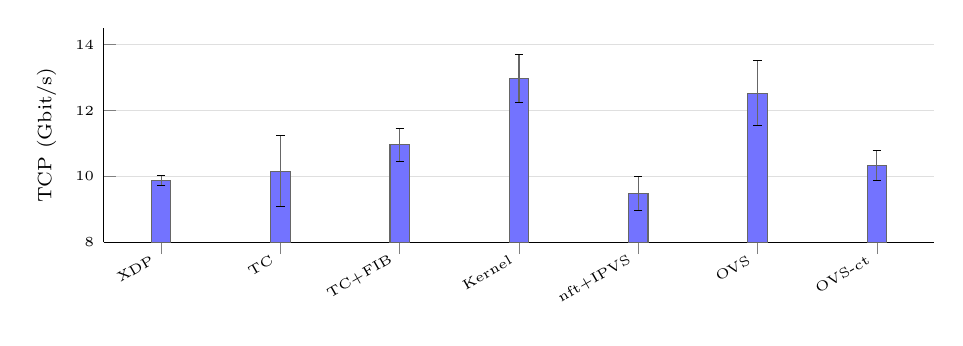
\begin{tikzpicture}
\begin{axis}[ybar, width=\linewidth, height=4.3cm, bar width=7pt,
  scaled y ticks=false, yticklabel style={/pgf/number format/fixed},
  symbolic x coords={XDP,TC,TC+FIB,Kernel,nft+IPVS,OVS,OVS-ct}, xtick=data, ymin=8, ymax=14.5,
  ylabel={TCP (Gbit/s)}, enlarge x limits=0.08, axis lines*=left,
  ymajorgrids, grid style={gray!25}, x tick label style={rotate=30, anchor=east, font=\tiny},
  y tick label style={font=\tiny}, label style={font=\scriptsize},
  error bars/y dir=both, error bars/y explicit]
\addplot[fill=blue!55, draw=black!60, error bars/.cd, y dir=both, y explicit, error mark options={rotate=90, mark size=1.5pt}] coordinates {(XDP,9.87) +- (0,0.155) (TC,10.16) +- (0,1.07) (TC+FIB,10.96) +- (0,0.506) (Kernel,12.97) +- (0,0.733) (nft+IPVS,9.487) +- (0,0.512) (OVS,12.53) +- (0,0.979) (OVS-ct,10.33) +- (0,0.461)};
\end{axis}
\end{tikzpicture}
\captionof{figure}{\textbf{Routed TCP throughput.} Routed-path TCP throughput, mean $\pm$ 95\% CI over 10 interleaved rounds. Axis starts at 8.}\label{fig:app-tcp}
\end{minipage}
\hfill
\begin{minipage}[t]{0.48\textwidth}\centering
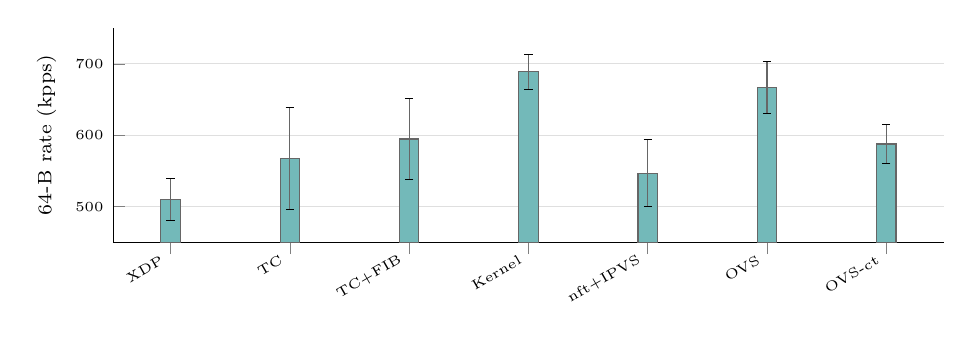
\begin{tikzpicture}
\begin{axis}[ybar, width=\linewidth, height=4.3cm, bar width=7pt,
  scaled y ticks=false, yticklabel style={/pgf/number format/fixed},
  symbolic x coords={XDP,TC,TC+FIB,Kernel,nft+IPVS,OVS,OVS-ct}, xtick=data, ymin=450, ymax=750,
  ylabel={64-B rate (kpps)}, enlarge x limits=0.08, axis lines*=left,
  ymajorgrids, grid style={gray!25}, x tick label style={rotate=30, anchor=east, font=\tiny},
  y tick label style={font=\tiny}, label style={font=\scriptsize},
  error bars/y dir=both, error bars/y explicit]
\addplot[fill=teal!55, draw=black!60, error bars/.cd, y dir=both, y explicit, error mark options={rotate=90, mark size=1.5pt}] coordinates {(XDP,510.5) +- (0,29.5) (TC,567.7) +- (0,71.4) (TC+FIB,594.8) +- (0,56.2) (Kernel,688.8) +- (0,24.5) (nft+IPVS,546.9) +- (0,47.1) (OVS,667) +- (0,36.8) (OVS-ct,587.8) +- (0,27.1)};
\end{axis}
\end{tikzpicture}
\captionof{figure}{\textbf{Routed packet rate.} Routed-path 64-byte packet rate, mean $\pm$ 95\% CI over 10 interleaved rounds. Axis starts at 450.}\label{fig:app-pps}
\end{minipage}
\par\vspace{2mm}
\begin{minipage}[t]{0.48\textwidth}\centering
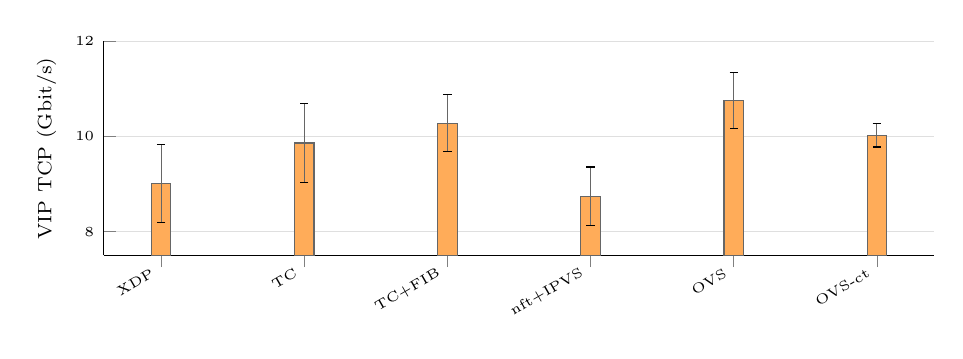
\begin{tikzpicture}
\begin{axis}[ybar, width=\linewidth, height=4.3cm, bar width=7pt,
  scaled y ticks=false, yticklabel style={/pgf/number format/fixed},
  symbolic x coords={XDP,TC,TC+FIB,nft+IPVS,OVS,OVS-ct}, xtick=data, ymin=7.5, ymax=12,
  ylabel={VIP TCP (Gbit/s)}, enlarge x limits=0.08, axis lines*=left,
  ymajorgrids, grid style={gray!25}, x tick label style={rotate=30, anchor=east, font=\tiny},
  y tick label style={font=\tiny}, label style={font=\scriptsize},
  error bars/y dir=both, error bars/y explicit]
\addplot[fill=orange!65, draw=black!60, error bars/.cd, y dir=both, y explicit, error mark options={rotate=90, mark size=1.5pt}] coordinates {(XDP,9.011) +- (0,0.822) (TC,9.863) +- (0,0.825) (TC+FIB,10.28) +- (0,0.603) (nft+IPVS,8.747) +- (0,0.612) (OVS,10.76) +- (0,0.587) (OVS-ct,10.03) +- (0,0.252)};
\end{axis}
\end{tikzpicture}
\captionof{figure}{\textbf{VIP TCP throughput.} TCP throughput through the load balancer (VIP path), mean $\pm$ 95\% CI over 10 interleaved rounds. Axis starts at 7.5.}\label{fig:app-viptcp}
\end{minipage}
\hfill
\begin{minipage}[t]{0.48\textwidth}\centering
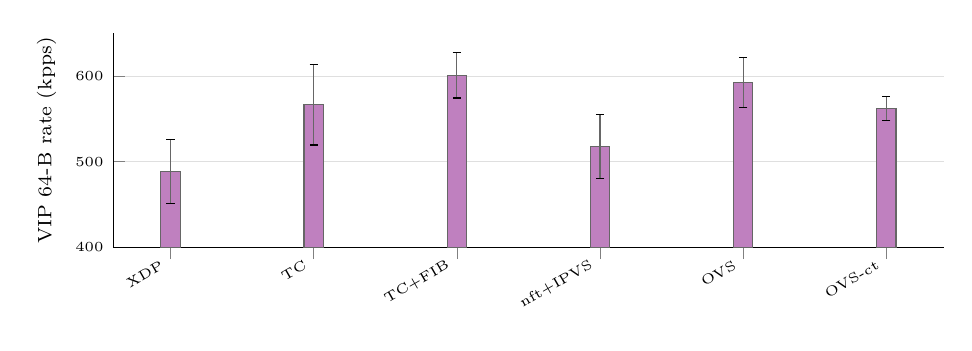
\begin{tikzpicture}
\begin{axis}[ybar, width=\linewidth, height=4.3cm, bar width=7pt,
  scaled y ticks=false, yticklabel style={/pgf/number format/fixed},
  symbolic x coords={XDP,TC,TC+FIB,nft+IPVS,OVS,OVS-ct}, xtick=data, ymin=400, ymax=650,
  ylabel={VIP 64-B rate (kpps)}, enlarge x limits=0.08, axis lines*=left,
  ymajorgrids, grid style={gray!25}, x tick label style={rotate=30, anchor=east, font=\tiny},
  y tick label style={font=\tiny}, label style={font=\scriptsize},
  error bars/y dir=both, error bars/y explicit]
\addplot[fill=violet!50, draw=black!60, error bars/.cd, y dir=both, y explicit, error mark options={rotate=90, mark size=1.5pt}] coordinates {(XDP,488.3) +- (0,37.2) (TC,566.5) +- (0,47) (TC+FIB,600.8) +- (0,26.4) (nft+IPVS,518) +- (0,37.2) (OVS,592.7) +- (0,29.1) (OVS-ct,562.1) +- (0,14.2)};
\end{axis}
\end{tikzpicture}
\captionof{figure}{\textbf{VIP packet rate.} 64-byte packet rate through the load balancer, mean $\pm$ 95\% CI over 10 interleaved rounds. Axis starts at 400.}\label{fig:app-vippps}
\end{minipage}
\par\vspace{2mm}
\begin{minipage}[t]{0.48\textwidth}\centering
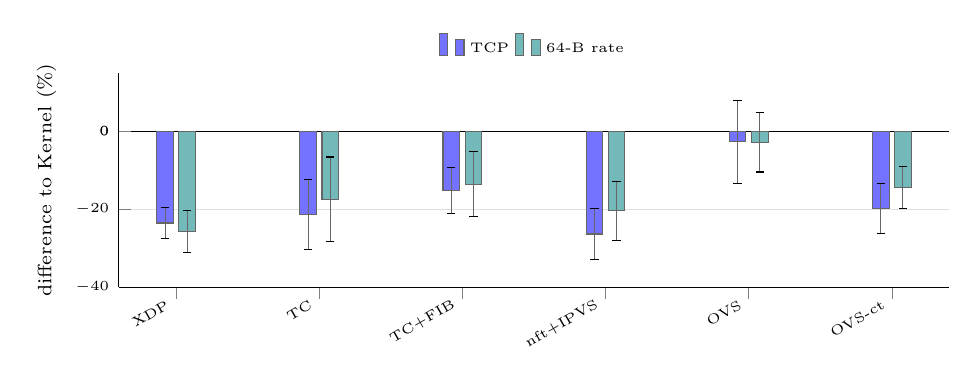
\begin{tikzpicture}
\begin{axis}[ybar, width=\linewidth, height=4.3cm, bar width=7pt,
  scaled y ticks=false, yticklabel style={/pgf/number format/fixed},
  symbolic x coords={XDP,TC,TC+FIB,nft+IPVS,OVS,OVS-ct}, xtick=data, ymin=-40, ymax=15,
  ylabel={difference to Kernel (\%)}, enlarge x limits=0.08, axis lines*=left,
  ymajorgrids, grid style={gray!25}, x tick label style={rotate=30, anchor=east, font=\tiny},
  y tick label style={font=\tiny}, label style={font=\scriptsize},
  error bars/y dir=both, error bars/y explicit, bar width=6pt, legend style={font=\tiny, at={(0.5,1.02)}, anchor=south, legend columns=2, draw=none}, extra y ticks={0}, extra y tick style={grid style={black, thin}}]
\addplot[fill=blue!55, draw=black!60, error bars/.cd, y dir=both, y explicit, error mark options={rotate=90, mark size=1.5pt}] coordinates {(XDP,-23.53) +- (0,3.98) (TC,-21.34) +- (0,8.89) (TC+FIB,-15.14) +- (0,5.88) (nft+IPVS,-26.36) +- (0,6.52) (OVS,-2.665) +- (0,10.7) (OVS-ct,-19.85) +- (0,6.49)};
\addplot[fill=teal!55, draw=black!60, error bars/.cd, y dir=both, y explicit, error mark options={rotate=90, mark size=1.5pt}] coordinates {(XDP,-25.69) +- (0,5.31) (TC,-17.38) +- (0,10.8) (TC+FIB,-13.55) +- (0,8.38) (nft+IPVS,-20.4) +- (0,7.52) (OVS,-2.787) +- (0,7.63) (OVS-ct,-14.41) +- (0,5.5)};
\legend{TCP, 64-B rate}
\end{axis}
\end{tikzpicture}
\captionof{figure}{\textbf{Paired difference to Kernel.} Cost relative to plain kernel routing: per-round paired relative difference, mean $\pm$ 95\% CI (paired $t$).}\label{fig:app-vskernel}
\end{minipage}
\hfill
\begin{minipage}[t]{0.48\textwidth}\centering
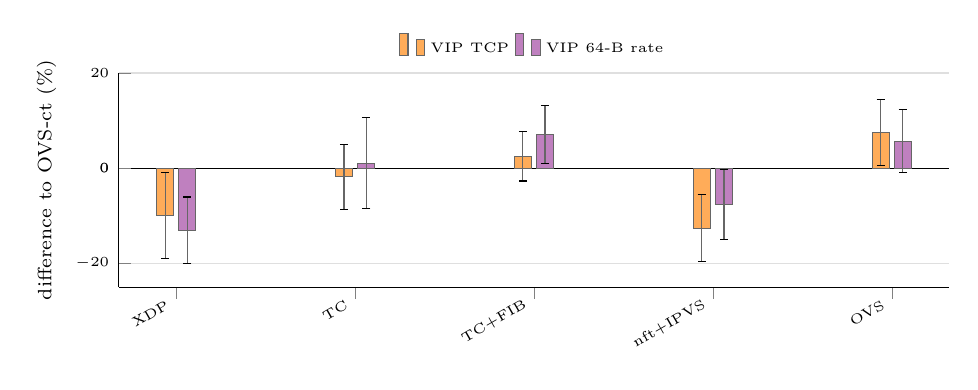
\begin{tikzpicture}
\begin{axis}[ybar, width=\linewidth, height=4.3cm, bar width=7pt,
  scaled y ticks=false, yticklabel style={/pgf/number format/fixed},
  symbolic x coords={XDP,TC,TC+FIB,nft+IPVS,OVS}, xtick=data, ymin=-25, ymax=20,
  ylabel={difference to OVS-ct (\%)}, enlarge x limits=0.08, axis lines*=left,
  ymajorgrids, grid style={gray!25}, x tick label style={rotate=30, anchor=east, font=\tiny},
  y tick label style={font=\tiny}, label style={font=\scriptsize},
  error bars/y dir=both, error bars/y explicit, bar width=6pt, legend style={font=\tiny, at={(0.5,1.02)}, anchor=south, legend columns=2, draw=none}, extra y ticks={0}, extra y tick style={grid style={black, thin}}]
\addplot[fill=orange!65, draw=black!60, error bars/.cd, y dir=both, y explicit, error mark options={rotate=90, mark size=1.5pt}] coordinates {(XDP,-9.965) +- (0,9) (TC,-1.83) +- (0,6.84) (TC+FIB,2.459) +- (0,5.16) (nft+IPVS,-12.6) +- (0,7.08) (OVS,7.504) +- (0,6.9)};
\addplot[fill=violet!50, draw=black!60, error bars/.cd, y dir=both, y explicit, error mark options={rotate=90, mark size=1.5pt}] coordinates {(XDP,-13.04) +- (0,6.98) (TC,1.034) +- (0,9.55) (TC+FIB,7.052) +- (0,6.04) (nft+IPVS,-7.686) +- (0,7.4) (OVS,5.644) +- (0,6.6)};
\legend{VIP TCP, VIP 64-B rate}
\end{axis}
\end{tikzpicture}
\captionof{figure}{\textbf{Paired difference to OVS-ct.} VIP-path performance relative to OVS-ct: per-round paired relative difference, mean $\pm$ 95\% CI (paired $t$).}\label{fig:app-vsovs}
\end{minipage}
\par\vspace{2mm}
\begin{minipage}[t]{0.48\textwidth}\centering
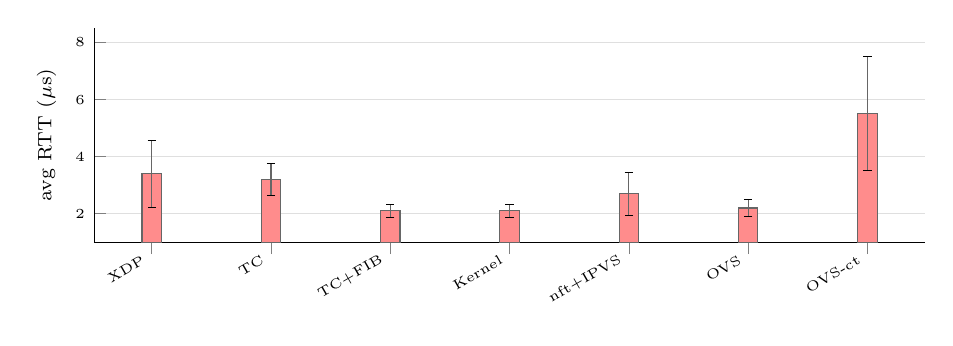
\begin{tikzpicture}
\begin{axis}[ybar, width=\linewidth, height=4.3cm, bar width=7pt,
  scaled y ticks=false, yticklabel style={/pgf/number format/fixed},
  symbolic x coords={XDP,TC,TC+FIB,Kernel,nft+IPVS,OVS,OVS-ct}, xtick=data, ymin=1, ymax=8.5,
  ylabel={avg RTT ($\mu$s)}, enlarge x limits=0.08, axis lines*=left,
  ymajorgrids, grid style={gray!25}, x tick label style={rotate=30, anchor=east, font=\tiny},
  y tick label style={font=\tiny}, label style={font=\scriptsize},
  error bars/y dir=both, error bars/y explicit]
\addplot[fill=red!45, draw=black!60, error bars/.cd, y dir=both, y explicit, error mark options={rotate=90, mark size=1.5pt}] coordinates {(XDP,3.4) +- (0,1.18) (TC,3.2) +- (0,0.564) (TC+FIB,2.1) +- (0,0.226) (Kernel,2.1) +- (0,0.226) (nft+IPVS,2.7) +- (0,0.758) (OVS,2.2) +- (0,0.302) (OVS-ct,5.5) +- (0,2)};
\end{axis}
\end{tikzpicture}
\captionof{figure}{\textbf{Average RTT.} Average round-trip time on the routed path, mean $\pm$ 95\% CI over 10 interleaved rounds. Axis starts at 1.}\label{fig:app-rtt}
\end{minipage}
\hfill
\begin{minipage}[t]{0.48\textwidth}\centering
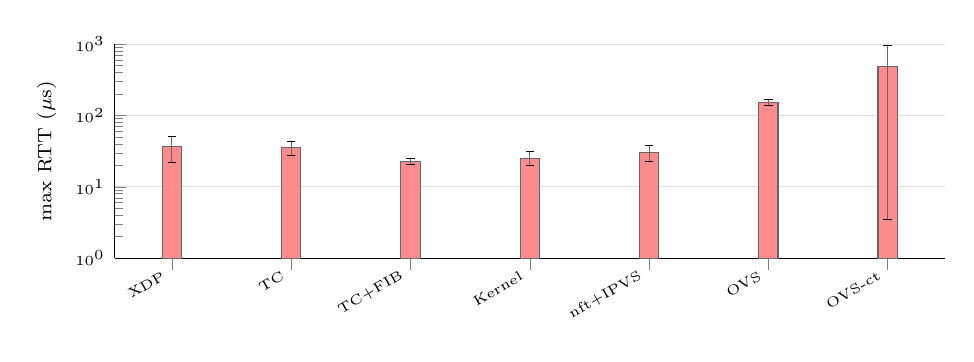
\begin{tikzpicture}
\begin{axis}[ybar, width=\linewidth, height=4.3cm, bar width=7pt,
  scaled y ticks=false, yticklabel style={/pgf/number format/fixed},
  symbolic x coords={XDP,TC,TC+FIB,Kernel,nft+IPVS,OVS,OVS-ct}, xtick=data, ymin=1, ymax=1000,
  ylabel={max RTT ($\mu$s)}, enlarge x limits=0.08, axis lines*=left,
  ymajorgrids, grid style={gray!25}, x tick label style={rotate=30, anchor=east, font=\tiny},
  y tick label style={font=\tiny}, label style={font=\scriptsize},
  error bars/y dir=both, error bars/y explicit, ymode=log, log origin=infty]
\addplot[fill=red!45, draw=black!60, error bars/.cd, y dir=both, y explicit, error mark options={rotate=90, mark size=1.5pt}] coordinates {(XDP,36.3) +- (0,14.3) (TC,35.3) +- (0,7.46) (TC+FIB,22.7) +- (0,2.16) (Kernel,25.3) +- (0,5.58) (nft+IPVS,30.1) +- (0,7.5) (OVS,151.5) +- (0,14) (OVS-ct,486.5) +- (0,483)};
\end{axis}
\end{tikzpicture}
\captionof{figure}{\textbf{Maximum RTT.} Maximum round-trip time on the routed path, mean $\pm$ 95\% CI over 10 interleaved rounds. Logarithmic axis.}\label{fig:app-rttmax}
\end{minipage}
\end{figure*}
\begin{figure*}[!p]\centering
\begin{minipage}[t]{0.48\textwidth}\centering
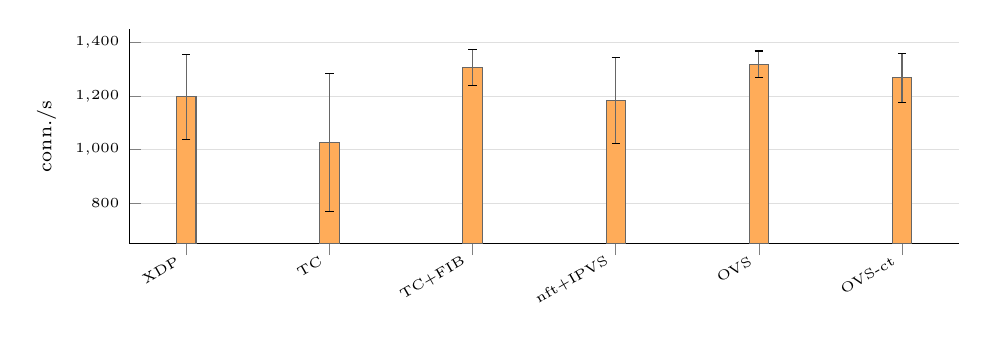
\begin{tikzpicture}
\begin{axis}[ybar, width=\linewidth, height=4.3cm, bar width=7pt,
  scaled y ticks=false, yticklabel style={/pgf/number format/fixed},
  symbolic x coords={XDP,TC,TC+FIB,nft+IPVS,OVS,OVS-ct}, xtick=data, ymin=650, ymax=1450,
  ylabel={conn./s}, enlarge x limits=0.08, axis lines*=left,
  ymajorgrids, grid style={gray!25}, x tick label style={rotate=30, anchor=east, font=\tiny},
  y tick label style={font=\tiny}, label style={font=\scriptsize},
  error bars/y dir=both, error bars/y explicit]
\addplot[fill=orange!65, draw=black!60, error bars/.cd, y dir=both, y explicit, error mark options={rotate=90, mark size=1.5pt}] coordinates {(XDP,1198) +- (0,159) (TC,1027) +- (0,259) (TC+FIB,1306) +- (0,67.3) (nft+IPVS,1183) +- (0,161) (OVS,1319) +- (0,50) (OVS-ct,1269) +- (0,92.2)};
\end{axis}
\end{tikzpicture}
\captionof{figure}{\textbf{VIP connection rate.} New-connection rate through the VIP (HTTP), mean $\pm$ 95\% CI over 10 interleaved rounds. Axis starts at 650.}\label{fig:app-lbrps}
\end{minipage}
\hfill
\begin{minipage}[t]{0.48\textwidth}\centering
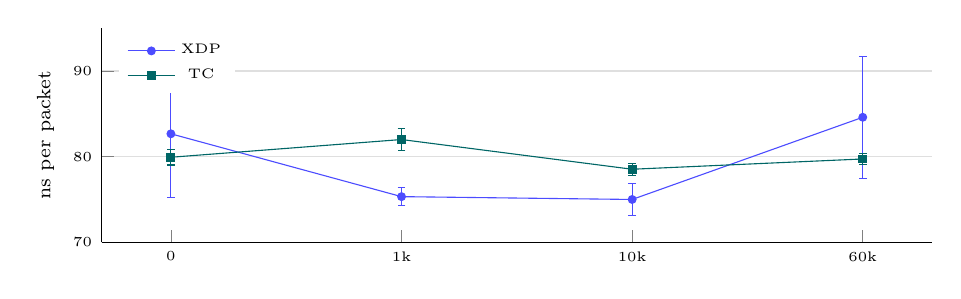
\begin{tikzpicture}
\begin{axis}[width=\linewidth, height=4.3cm, scaled y ticks=false, symbolic x coords={0,1k,10k,60k}, xtick=data, ymin=70, ymax=95, ylabel={ns per packet},
  axis lines*=left, ymajorgrids, grid style={gray!25}, tick label style={font=\tiny}, label style={font=\scriptsize},
  legend style={font=\tiny, at={(0.02,0.98)}, anchor=north west, draw=none}]
\addplot[blue!70, mark=*, mark size=1.4pt, error bars/.cd, y dir=both, y explicit] coordinates {(0,82.67) +- (0,7.45) (1k,75.33) +- (0,1.08) (10k,75) +- (0,1.88) (60k,84.6) +- (0,7.1)};
\addplot[teal!80!black, mark=square*, mark size=1.4pt, error bars/.cd, y dir=both, y explicit] coordinates {(0,79.93) +- (0,0.9) (1k,82) +- (0,1.29) (10k,78.53) +- (0,0.721) (60k,79.73) +- (0,0.677)};
\legend{XDP, TC}
\end{axis}
\end{tikzpicture}
\captionof{figure}{\textbf{Connection-table scaling.} In-kernel cost of an admitted packet versus tracked connections per table (empty rule tables), zoomed view of Fig.~\ref{fig:scale}; mean $\pm$ 95\% CI of 15 repeat-loop samples.}\label{fig:app-conntrack}
\end{minipage}
\par\vspace{2mm}
\begin{minipage}[t]{0.48\textwidth}\centering
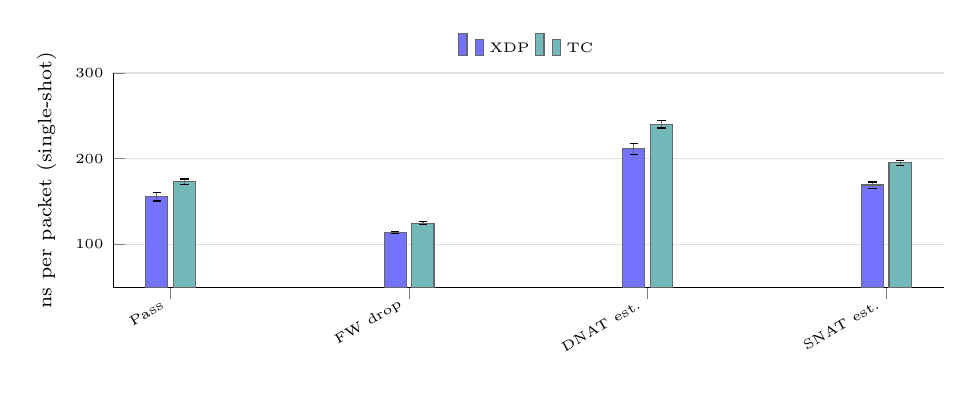
\begin{tikzpicture}
\begin{axis}[ybar, width=\linewidth, height=4.3cm, bar width=7pt,
  scaled y ticks=false, yticklabel style={/pgf/number format/fixed},
  symbolic x coords={Pass,FW drop,DNAT est.,SNAT est.}, xtick=data, ymin=50, ymax=300,
  ylabel={ns per packet (single-shot)}, enlarge x limits=0.08, axis lines*=left,
  ymajorgrids, grid style={gray!25}, x tick label style={rotate=30, anchor=east, font=\tiny},
  y tick label style={font=\tiny}, label style={font=\scriptsize},
  error bars/y dir=both, error bars/y explicit, bar width=8pt, legend style={font=\tiny, at={(0.5,1.02)}, anchor=south, legend columns=2, draw=none}]
\addplot[fill=blue!55, draw=black!60, error bars/.cd, y dir=both, y explicit, error mark options={rotate=90, mark size=1.5pt}] coordinates {(Pass,155.7) +- (0,5.09) (FW drop,113.6) +- (0,1.31) (DNAT est.,211.5) +- (0,6.33) (SNAT est.,169.2) +- (0,3.57)};
\addplot[fill=teal!55, draw=black!60, error bars/.cd, y dir=both, y explicit, error mark options={rotate=90, mark size=1.5pt}] coordinates {(Pass,173) +- (0,3.2) (FW drop,124.6) +- (0,1.79) (DNAT est.,240.3) +- (0,4.42) (SNAT est.,195.2) +- (0,2.84)};
\legend{XDP, TC}
\end{axis}
\end{tikzpicture}
\captionof{figure}{\textbf{Per-path cost by hook.} In-kernel single-shot cost per processing path at the XDP and TC hooks with one installed rule; mean $\pm$ 95\% CI of 10 batch means. Axis starts at 50.}\label{fig:app-paths}
\end{minipage}
\hfill
\begin{minipage}[t]{0.48\textwidth}\centering
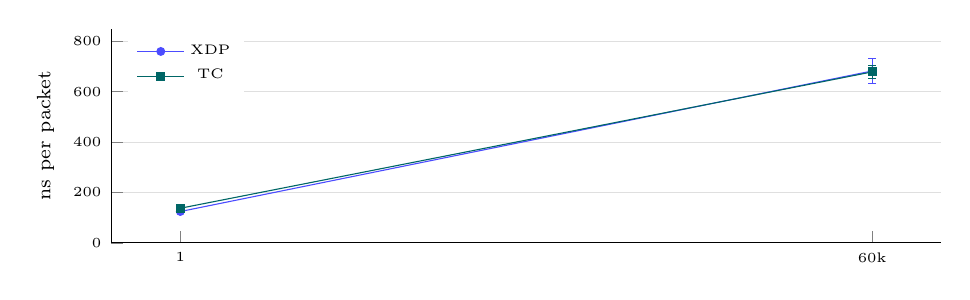
\begin{tikzpicture}
\begin{axis}[width=\linewidth, height=4.3cm, scaled y ticks=false, symbolic x coords={1,1k,15k,60k,60k}, xtick=data, ymin=0, ymax=850, ylabel={ns per packet},
  axis lines*=left, ymajorgrids, grid style={gray!25}, tick label style={font=\tiny}, label style={font=\scriptsize},
  legend style={font=\tiny, at={(0.02,0.98)}, anchor=north west, draw=none}]
\addplot[blue!70, mark=*, mark size=1.4pt, error bars/.cd, y dir=both, y explicit] coordinates {(1,124.3) +- (0,3.92) (60k,682.4) +- (0,50.3)};
\addplot[teal!80!black, mark=square*, mark size=1.4pt, error bars/.cd, y dir=both, y explicit] coordinates {(1,137.3) +- (0,3.86) (60k,678.7) +- (0,25.3)};
\legend{XDP, TC}
\end{axis}
\end{tikzpicture}
\captionof{figure}{\textbf{Cache-cold cost.} In-kernel single-shot cost versus the number of tracked flows visited in random order (cache-cold); mean $\pm$ 95\% CI of 10 batch means.}\label{fig:app-cold}
\end{minipage}
\par\vspace{2mm}
\begin{minipage}[t]{0.48\textwidth}\centering
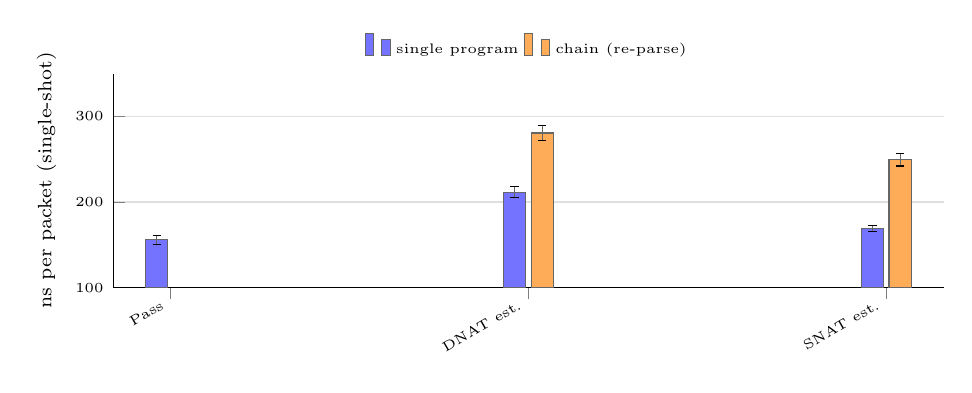
\begin{tikzpicture}
\begin{axis}[ybar, width=\linewidth, height=4.3cm, bar width=7pt,
  scaled y ticks=false, yticklabel style={/pgf/number format/fixed},
  symbolic x coords={Pass,DNAT est.,SNAT est.}, xtick=data, ymin=100, ymax=350,
  ylabel={ns per packet (single-shot)}, enlarge x limits=0.08, axis lines*=left,
  ymajorgrids, grid style={gray!25}, x tick label style={rotate=30, anchor=east, font=\tiny},
  y tick label style={font=\tiny}, label style={font=\scriptsize},
  error bars/y dir=both, error bars/y explicit, bar width=8pt, legend style={font=\tiny, at={(0.5,1.02)}, anchor=south, legend columns=3, draw=none}]
\addplot[fill=blue!55, draw=black!60, error bars/.cd, y dir=both, y explicit, error mark options={rotate=90, mark size=1.5pt}] coordinates {(Pass,155.7) +- (0,5.09) (DNAT est.,211.5) +- (0,6.33) (SNAT est.,169.2) +- (0,3.57)};
\addplot[fill=orange!65, draw=black!60, error bars/.cd, y dir=both, y explicit, error mark options={rotate=90, mark size=1.5pt}] coordinates {(DNAT est.,280.5) +- (0,8.99) (SNAT est.,249.3) +- (0,7.25)};
\legend{single program, chain (re-parse)}
\end{axis}
\end{tikzpicture}
\captionof{figure}{\textbf{Tail-call ablation.} Tail-call ablation (XDP): single program versus the same stages chained with tail calls; mean $\pm$ 95\% CI of 10 batch means. Axis starts at 100.}\label{fig:app-chain}
\end{minipage}
\hfill
\begin{minipage}[t]{0.48\textwidth}\centering
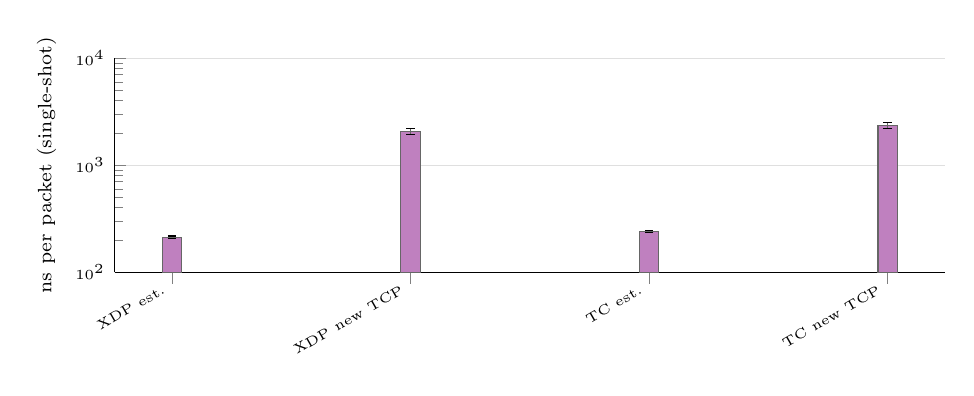
\begin{tikzpicture}
\begin{axis}[ybar, width=\linewidth, height=4.3cm, bar width=7pt,
  scaled y ticks=false, yticklabel style={/pgf/number format/fixed},
  symbolic x coords={XDP est.,XDP new TCP,TC est.,TC new TCP}, xtick=data, ymin=100, ymax=10000,
  ylabel={ns per packet (single-shot)}, enlarge x limits=0.08, axis lines*=left,
  ymajorgrids, grid style={gray!25}, x tick label style={rotate=30, anchor=east, font=\tiny},
  y tick label style={font=\tiny}, label style={font=\scriptsize},
  error bars/y dir=both, error bars/y explicit, ymode=log, log origin=infty]
\addplot[fill=violet!50, draw=black!60, error bars/.cd, y dir=both, y explicit, error mark options={rotate=90, mark size=1.5pt}] coordinates {(XDP est.,211.5) +- (0,6.33) (XDP new TCP,2065) +- (0,118) (TC est.,240.3) +- (0,4.42) (TC new TCP,2361) +- (0,157)};
\end{axis}
\end{tikzpicture}
\captionof{figure}{\textbf{New-connection cost.} In-kernel cost of DNAT for an established connection and for a new connection (and a new UDP flow, where measured); mean $\pm$ 95\% CI. Logarithmic axis.}\label{fig:app-newconn}
\end{minipage}
\end{figure*}
\clearpage  % flush the figure pages before the references
